\section{Auswertung des \sarsa Agenten}
In den folgenden Abschnitten werden die Ergebnisse der Sarsa Agenten vorgestellt und ausgewertet. Zunächst wird die Konvergenz während dem Training und die Spielstärke betrachtet. Anschließend wird vorgestellt, welche Auswirkung die Nutzung von Afterstates hat. Abschließend erfolgt eine Detailbetrachtung für ausgewählte Zustände.
\subsection{Konvergenz der Rate optimaler Aktionen}

\begin{figure}
\centering
\begin{subfigure}[b]{0.75\textwidth}
    \centering
   \includegraphics[width=1\linewidth]{convergence/convergence_compare_alpha_sarsa_X.pdf}
   \caption{Symbol X}
   \label{fig:convergence_compare_alpha_sarsa_X} 
\end{subfigure}

\begin{subfigure}[b]{0.75\textwidth}
    \centering
   \includegraphics[width=1\linewidth]{convergence/convergence_compare_alpha_sarsa_O.pdf}
   \caption{Symbol O}
   \label{fig:convergence_compare_alpha_sarsa_O}
\end{subfigure}

\caption[Rate optimaler Aktionen \sarsa unterschiedliche Lernraten, klassisches \splay]{Rate optimaler Aktionen von \sarsa für verschiedene Lernraten $\alpha$, klassisches \splay (a) Symbol X (b) Symbol O}
\label{fig:convergence_compare_alpha_sarsa}
\end{figure}

\cref{fig:convergence_compare_alpha_sarsa} zeigt den Verlauf der Rate optimaler Aktionen von \sarsa Agenten mit den drei verschiedenen Lernraten $\alpha$ während des Trainings mit klassischem \splay. 
Der Agent mit Lernrate $\alpha=0,1$ konvergiert am schnellsten, dicht gefolgt von $\alpha=0,2$. 
Für das Symbol X stabilisiert sich die Rate ab ungefähr 90.000 und für O ab 110.000 Trainingsepisoden. 

Die Agenten von Symbol X stabilisieren sich auf einer höheren Rate optimaler Aktionen als die von Symbol O, wobei in beiden Fällen der Agent mit $\alpha=0,1$ die höchste Rate erreicht. 
Hingegen konvergiert bei beiden Symbolen der Agent mit abnehmender Lernrate langsamer und erreicht, insbesondere bei Symbol O, eine niedrigere Rate optimaler Aktionen.

Der Vergleich der Rate optimaler Aktionen von \sarsa für alternierendes \splay ist im \cref{chap:app_sarsa}. 
Für beide Symbole konvergiert das alternierende \splay langsamer als das klassische \splay und stabilisiert sich auf einer geringeren Rate.


\subsection{Spielstärke}
\cref{tab:playingAbility_sarsa_normal} und \cref{tab:playingAbility_sarsa_alternate} zeigen die durchschnittliche Spielstärke der trainierten Agenten für klassisches und alternierendes \splay. Für beide Arten von \splay erreichen die Agenten eine durchschnittliche Spielstärke, die über der des Minimax liegt. 
Die einzige Ausnahme sind Agenten, die mit konstanter Lernrate $\alpha=0,1$ durch alternierendes \splay trainiert wurden und eine durchschnittliche Spielstärke von 6.496,50 haben. 
Training durch klassisches \splay resultiert für \sarsa in stärkeren Agenten als Training durch alternierendes \splay. 
Der \sarsa Agent, der die Lernrate $\alpha=0,1$ nutzt und mit klassischem \splay trainiert wurde erreicht mit 7.905,72 die höchste Spielstärke. 

\cref{tab:resultmatrix_sarsa_normal_alpha01} enthält die Spielergebnisse der Evaluationsspiele des stärksten \sarsa Agenten. 
Als Symbol X spielt der \sarsa Agent optimal gegen Minimax. 
Zudem gewinnt der Agent 99\% der Spiele gegen Random und somit mehr als der Minimax, der nur 97\% gewinnt. 
Als Symbol O gewinnt der Agent mit 89\% mehr Spiele gegen Random als Minimax, der nur eine Gewinnrate von 78\% erreicht.
Jedoch verliert der Agent als Symbol O 0,74\% der Evaluationsspiele gegen Minimax und 0,11\% gegen Random.
Somit erreicht der Agent eine höhere Spielstärke als Minimax, spielt jedoch nicht optimal. 
Die Spielergebnismatrizen der \sarsa Agenten für die anderen Hyperparameter und Arten von \splay sind im \cref{chap:app_sarsa} angegeben.

\begin{table}
\centering
\caption[Spielstärke \sarsa unterschiedliche Lernraten, klassisches \splay]{Spielstärke von \sarsa mit unterschiedlichen Lernraten, klassisches \splay}
\label{tab:playingAbility_sarsa_normal}

% change color with \textcolor{red}{text}
\begin{tabular}{lrrr}
\toprule
Lernrate $\alpha$ &  Spielst"arke Sarsa & Spielst"arke Minimax & Differenz zu Minimax \\ \midrule
Konstant 0,1                    & 7.905,72 $\pm$ \phantom{0}75,69   & 6.917,86  & 987,86 $\pm$ \phantom{0}75,69 \\
Konstant 0,2                    & 7.787,94 $\pm$ 105,20             & 6.917,86  & 870,08 $\pm$ 105,20 \\
Abnehmend 1 $\rightarrow$ 0,1   & 7.754,66 $\pm$ 197,59             & 6.917,86  & 836,80 $\pm$ 197,59 \\ \bottomrule

\end{tabular}
\end{table}
\begin{table}
\centering
\caption[Spielstärke \sarsa unterschiedliche Lernraten, alternierendes \splay]{Spielstärke von \sarsa mit unterschiedlichen Lernraten, alternierendes \splay}
\label{tab:playingAbility_sarsa_alternate}

\begin{tabular}{lrrr}
\toprule
Lernrate $\alpha$ &  Spielst"arke Sarsa & Spielst"arke Minimax & Differenz zu Minimax \\ \midrule
Konstant 0,1                    & 6.495,50 $\pm$ 826,74             & 6.917,86      & \textcolor{red}{-422,36 $\pm$ 826,74} \\
Konstant 0,2                    & 7.018,94 $\pm$ 299,04             & 6.917,86      & 101,08 $\pm$ 299,04 \\
Abnehmend 1 $\rightarrow$ 0,1   & 7.625,94 $\pm$ \phantom{0}65,10   & 6.917,86      & 708,08 $\pm$ \phantom{0}65,10 \\ \bottomrule

\end{tabular}

\end{table}
\begin{table}
\centering
\caption[Spielergebnismatrix \sarsa: $\alpha=0,1$, klassisches \splay]{Spielergebnismatrix für \sarsa mit Lernrate $\alpha=0,1$, klassisches \splay}
\label{tab:resultmatrix_sarsa_normal_alpha01}

\begin{tabular}{llrlr}
\toprule
 & \multicolumn{2}{l}{\textbf{Minimax}} & \multicolumn{2}{l}{\textbf{Random}} \\ \midrule
\textbf{X Sarsa}        & X Sarsa:          & 0,00\% $\pm$    0,00\%            & X Sarsa:              & 99,01\% $\pm$ 0,04\%  \\
                        & O Minimax:        & 0,00\% $\pm$    0,00\%            & O Random:            & 0,00\% $\pm$ 0,00\%  \\
                        & Unentschieden:    & 100,00\% $\pm$  0,00\%            & Unentschieden:        & 0,99\% $\pm$ 0,04\%  \\ \cmidrule{2-5}
\textbf{O Sarsa}        & X Minimax:        & 0,74\% $\pm$    1,48\%            & X Random:             & 0,11\% $\pm$ 0,22\%  \\
                        & O Sarsa:          & 0,00\% $\pm$    0,00\%            & O Sarsa:              & 89,69\% $\pm$ 0,38\%  \\
                        & Unentschieden:    & 99,26\% $\pm$  1,48\%             & Unentschieden:        & 10,205\% $\pm$ 0,30\%  \\ \bottomrule
\end{tabular}
\end{table}

\subsection{\wtable}
\cref{fig:convergence_compare_experience_sarsa} vergleicht die Rate optimaler Aktionen des besten \sarsa Agenten mit \qtable und \wtable. 
Sowohl für Symbol X als auch für Symbol O konvergiert der Agent mit \wtable schneller und erreicht eine höhere Rate. 

\cref{tab:resultmatrix_sarsa_normal_alpha01_afterstate} zeigt die Spielergebnismatrix des \sarsa Agenten mit \wtable. 
Im Gegensatz zum Agenten mit \qtable verliert der Agent keine Spiele mehr und spielt optimal gegen Minimax. 
Die Gewinnrate gegen Random bleibt für das Symbol X unverändert bei 99\%. 
Für das Symbol O sinkt die Gewinnrate von 89,69\% auf 88,61\%. 
Die durchschnittliche Spielstärke des Agenten steigt durch die Nutzung des \wtable von 7.905,72 auf 7.927,68.
Da die Standardabweichung für die Spielstärke des Agenten mit \qtable jedoch $\pm 30,03$ beträgt und die Stichprobenanzahl mit $N=5$ klein ist, kann dies nicht sicher gesagt werden.
Es ist daher auch möglich, dass die Verbesserung durch Zufall entstanden somit statistisch nicht signifikant ist.

\begin{figure}
\centering
\begin{subfigure}[b]{0.75\textwidth}
    \centering
   \includegraphics[width=1\linewidth]{convergence/convergence_compare_experience_sarsa_X.pdf}
   \caption{Symbol X}
   \label{fig:convergence_compare_experience_sarsa_X} 
\end{subfigure}

\begin{subfigure}[b]{0.75\textwidth}
    \centering
   \includegraphics[width=1\linewidth]{convergence/convergence_compare_experience_sarsa_O.pdf}
   \caption{Symbol O}
   \label{fig:convergence_compare_experience_sarsa_O}
\end{subfigure}
\caption[Rate optimaler Aktionen bester \sarsa Agent, \wtable, klassisches \splay]{Rate optimaler Aktionen von \sarsa Lernrate $\alpha=0,1$, \wtable, klassisches \splay (a) Symbol X (b) Symbol O}
\label{fig:convergence_compare_experience_sarsa}
\end{figure}

\begin{table}
\centering
\caption[Spielergebnismatrix \sarsa: $\alpha=0,1$, \wtable, klassisches \splay]{Spielergebnismatrix für \sarsa mit Lernrate $\alpha=0,1$ und \wtable, klassisches \splay}
\label{tab:resultmatrix_sarsa_normal_alpha01_afterstate}

\begin{tabular}{llrlr}
\toprule
 & \multicolumn{2}{l}{\textbf{Minimax}} & \multicolumn{2}{l}{\textbf{Random}} \\ \midrule
\textbf{X Sarsa}        & X Sarsa:          & 0,00\% $\pm$    0,00\%            & X Sarsa:              & 99,01\% $\pm$ 0,83\%  \\
                        & O Minimax:        & 0,00\% $\pm$    0,00\%            & O Random:            & 0,00\% $\pm$ 0,00\%  \\
                        & Unentschieden:    & 100,00\% $\pm$  0,00\%            & Unentschieden:        & 0,98\% $\pm$ 0,83\%  \\ \cmidrule{2-5}
\textbf{O Sarsa}        & X Minimax:        & 0,00\% $\pm$    0,00\%            & X Random:             & 0,00\% $\pm$ 0,00\%  \\
                        & O Sarsa:          & 0,00\% $\pm$    0,00\%            & O Sarsa:              & 88,61\% $\pm$ 1,28\%  \\
                        & Unentschieden:    & 100,00\% $\pm$  0,00\%            & Unentschieden:        & 11,39\% $\pm$ 1,28\%  \\ \bottomrule
\end{tabular}
\end{table}

\subsection{Detailbetrachtung}
Obwohl die Spielstärke der trainierten \sarsa Agenten über dem Minimax liegt, verliert der beste Agent mit \qtable als Symbol O. 
Ein Zustand, der in den Evaluationsspielen mehrfach für eine Niederlage als Symbol O sorgte ist $69648$, der in \cref{ttt_boards/ttt_69648} dargestellt ist. 
Die optimalen Aktionen laut Minimax und Expert Play sind 0, 6 und 8, um den Gegner zum Blocken zu zwingen. 
Der Agent mit \qtable wählt jedoch gemäß Greedy-Strategie die nicht optimale Aktion 5, da diese nach Abschluss des Trainings den höchsten \qValue hat. 
Die \qtable zeigt jedoch, dass die optimalen Aktionen im Vergleich zu den anderen Aktionen die höheren \qValues haben. 
Lediglich der \qValue für die Aktion 5 ist leicht höher. 
Der Agent benötigt demnach noch mehr Trainingsepisoden, um den Aktionen die richtige Bewertung zuzuweisen. 
Dies bestätigt sich, wenn der \sarsa Agent mit der \wtable trainiert wird, um die gesammelte Erfahrung effektiver zu nutzen.  
Durch Nutzung der \wtable ändert sich die Bewertung der Aktionen und die optimalen Aktionen 0, 6 und 8 haben nun die höchsten \qValues.

\begin{minipage}{\textwidth}
  \begin{minipage}[t]{0.49\textwidth}
    \centering
    \captionsetup{type=figure}
    \captionof{figure}{Spielfeldkonstellation Zustand 69648}
    \label{ttt_boards/ttt_69648}
    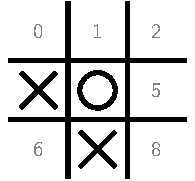
\includegraphics[]{ttt_boards/ttt_69648.pdf}
  \end{minipage}
  \hfill
  \begin{minipage}[t]{0.49\textwidth}
    \centering
    \captionsetup{type=table}
    \captionof{table}{Bewertung Aktionen in Zustand 69648}
    \label{tab:state69648}
    %\begin{table}
%\centering
%\caption{Bewertung Aktionen in Zustand $69648_{10}$}
\begin{tabular}{lrr}
\toprule
Aktion  & Q-Tabelle& W-Tabelle\\ \midrule
0   	& -0,0008	        & 0,0016  \\
1	    & -0,0851	        & -0,1470 \\
2	    & -0,0300       	& -0,1466 \\
5	    & 0,0013	        & -0,1658 \\
6	    & 0,0002        	& 0,0069  \\
8	    & -0,0038	        & 0,0016  \\ \bottomrule
\end{tabular}
%\end{table}
    \end{minipage}
\end{minipage}

Zur Prüfung welche Aktion laut den trainierten \sarsa Agenten die beste erste Aktion für Symbol X ist, wird die durchschnittliche Bewertung von fünf Agenten betrachtet, die in \cref{tab:state0_eval_sarsa} gelistet sind. 
Alle Aktionen, mit Ausnahme der Aktion 4, haben ein negatives Vorzeichen.
Wie die obige Auswertung der Spielstärke der \wtable Agenten zeigt, behindert dies jedoch nicht die Spielstärke des Agenten, da bei der Aktionsauswahl lediglich die Aktion mit dem höchsten \qValue gewählt wird. 
In \cref{tab:state0_eval_sarsa_aggregated} wird die durchschnittliche Bewertung je äquivalenter Aktion betrachtet.
Laut den trainierten Sarsa Agenten ist die Rangfolge der Aktionen: Mitte, Ecke und Kante. 

\begin{table}[!htb]
    \begin{minipage}[t]{.49\textwidth}
        \centering
        \label{tab:state0_eval_sarsa}
        \caption{Bewertung Zustand 0 \\ bester Sarsa Agent}
        \begin{tabular}{lr}
        \toprule
        Aktion  & Bewertung \\ \midrule
        0	& -0,0283 \\
        1	& -0,0258 \\
        2	& -0,0223 \\
        3	& -0,0272 \\
        4	& 0,0019  \\
        5	& -0,0218 \\
        6	& -0,0337 \\
        7	& -0,0394 \\
        8	& -0,0274 \\ \bottomrule
        
        \end{tabular}
    \end{minipage}%
    \begin{minipage}[t]{.49\textwidth}
        \centering
        \caption{Bewertung Aktionsklassen Zustand 0 bester Sarsa Agent}
        \label{tab:state0_eval_sarsa_aggregated}
        \begin{tabular}{lr}
        \toprule
        Aktion  & Bewertung \\ \midrule
        Ecke	& -0,0279 \\
        Kante	& -0,0286 \\
        Mitte	&  0,0019 \\ \bottomrule
        
        \end{tabular}
    \end{minipage}
\end{table}